\documentclass[letterpaper,10pt]{article}
\usepackage[margin=2cm]{geometry}

\usepackage{graphicx}
\usepackage{amsmath}
\usepackage{amsfonts}
\usepackage{amssymb}
\usepackage[colorlinks]{hyperref}

\setlength{\parindent}{0em}
\setlength{\parskip}{0.3em}

\newcommand{\panhline}{\begin{center}\rule{\textwidth}{1pt}\end{center}}

\title{\textbf{Parametric Models: Prior Information, From Models to Answers}}
\author{Praddep Ravikumar (Instructor), HMW-Alexander (Noter)}

\begin{document}

\maketitle

\panhline
\href{../index.html}{Back to Index}

\panhline
\tableofcontents

\section*{Resources}

\begin{itemize}
	\item \href{../../Lectures/03_ParametricModels.pdf}{Lecture}
\end{itemize}

\panhline

\section{Bayesian Learning}

Given a prior knowledge to estimate the model.

Bayesian Learning:
$$P(\theta|\mathcal{D}) = \frac{P(\mathcal{D}|\theta)P(\theta)}{P(\mathcal{D})}$$
or equivalently
$$P(\theta|\mathcal{D}) \propto P(\mathcal{D}|\theta)P(\theta)$$
Likelihood measures the fitness between data and parameters, Prior is the knowledge how possible the parameters to be.

\begin{itemize}
	\item Prior information encoded as a distribution over possible values of parameter.
	\item Using the Bayes rule to get an updated posterior distribution over parameters.
\end{itemize}

\subsection{Prior Distribution}

\subsubsection{Where to get}

\begin{itemize}
	\item Represents expert knowledge (philosophical approach)
	\item Simple posterior form (engineer's approach)
\end{itemize}

\subsubsection{Uniformative priors}

Simple distribution. 
\begin{figure}[!h]
	\centering
	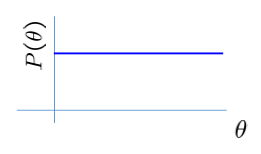
\includegraphics[width=4cm]{./img/uniform.png}
\end{figure}

\subsubsection{Conjugate Priors}

\begin{itemize}
	\item Closed-form representation of posterior
	\item prior and posterior have the same algebraic form as a function of parameters
\end{itemize}

Bernoulli Example: (Binomial's conjugate prior is Beta distribution)
\begin{itemize}
	\item Likelihood in Bernoulli model: $P(D|\theta)=\theta^{\alpha_1}(1-\theta)^{\alpha_2}$
	\item Prior is Beta distribution: $P(\theta)=\frac{\theta^{\beta_1-1}(1-\theta)^{\beta_2-1}}{B(\beta_1,\beta_2)} \sim Beta(\beta_1,\beta_2)$
	\item Posterior is also Beta distribution: $P(\theta|D)\sim Beta(\beta_1+\alpha_1,\beta_2+\alpha_2)$
\end{itemize}

Multinomial example: (Multinomial's conjugate prior is Dirichelet distribution)
\begin{itemize}
	\item Likelihood is Multinomial($\theta=\{\theta_1,\dots,\theta_k\}$), $P(D|\theta)=\prod_{i=1}^{k}\theta_i^{\alpha_i}$, $\alpha_i\in\{0,1\}$ is the data $D$, $\sum_{i=1}^{k}\theta_i =1$.
	\item Prior is Dirichlet distribution: $P(\theta)=\frac{\prod_{i=1}^{k}\theta_i^{\beta_i-1}}{B(\beta_1,\dots,\beta_k)} \sim Dirichlet(\beta_1,\dots,\beta_k)$
	\item Posterior is also dirichlet distribution: $P(\theta|D) \sim Dirichlet(\beta_1+\alpha_1,\dots,\beta_k+\alpha_k)$
\end{itemize}

As we get more samples, effect of prior is "washed out"

\section{Maximum A Posteriori Estimation}

Choose $\theta$ that maximizes a posterior probability:
$\hat{\theta}_{MAP}=\arg\max_\theta{P(\theta|D)}$

\begin{equation}
\begin{array}{rcl}
\hat{\theta}_{MAP} & = & \arg\max_\theta{P(\theta|D)} \\
				   & = & \arg\max_\theta{P(D|\theta)P(\theta)}
\end{array}
\end{equation}

Bernoulli example:

\begin{equation}
\begin{array}{rcl}
P(\theta|D) & \sim & Beta(\beta_1+\alpha_1,\beta_2+\beta_2) \\
\hat{\theta}_{MAP} & = & \frac{\alpha_1+\beta_1-1}{\alpha_1+\beta_1+\alpha_2+\beta_2-2}
\end{array}
\end{equation}

\subsection{MLE vs. MAP}

\begin{itemize}
	\item MLE: Choose value that maximizes the probability of observed data
	\item MAP: Choose value that is mot probable given observed data and prior belief
	\item When prior is a uniform distribution, MLE=MAP.
\end{itemize}

\subsection{MAP for Gaussian mean and variance}

Conjugate priors
\begin{itemize}
	\item Gaussian prior: $$P(\mu|\eta,\lambda)=\frac{1}{\lambda\sqrt{2\pi}}\exp(-\frac{(\mu-\eta)^2}{2\lambda^2})=\mathcal{N}(\eta,\lambda)$$
	\item Variance: Wishart Distribution\footnote{\url{https://en.wikipedia.org/wiki/Wishart_distribution}}
\end{itemize}

MAP for Gasussian Mean:
\begin{itemize}
	\item $\hat{\mu}_{MLE}=\frac{1}{n}\sum_{i=1}^{n}x_i$
	\item $\hat{\mu}_{MAP}=\frac{\frac{1}{\sigma^2}\sum_{i=1}^{n}x_i+\frac{\eta}{\lambda^2}}{\frac{n}{\sigma^2}+\frac{1}{\lambda^2}}$
\end{itemize}

\section{Non-Bayesian Prior Information via Constraints}

\begin{itemize}
	\item MLE: $$\max_\theta\log P(D|\theta)$$
	\item Constrained MLE: $$\max _\theta\log P(D|\theta)~~s.t.~\mathcal{R}(\theta)\leq C$$
	\item When $\mathcal{R}$ is convex, constrained MLE is equivalent to regularized MLE (lagrange multiplier\footnote{\url{http://www1.maths.leeds.ac.uk/~cajones/math2640/notes4.pdf}}): $$\max_\theta\{\log P(D|\theta)+\lambda\mathcal{R}(\theta)\}$$
	\item The MAP estimator can be seen to be a special case by simply setting: $$\lambda\mathcal{R}(\theta)=\log P(\theta)$$
\end{itemize}

\end{document}



